
\begin{figure}[!t]
    \centering
    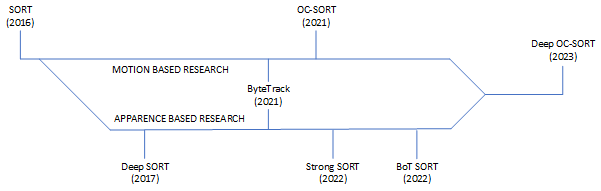
\includegraphics[width=0.9\linewidth]{figures/04_state_of_the_art/cronologia_sort.png}
    \caption[SORT algorithms timeline]{\footnotesize{Timeline of some \ac{SORT} based algorithms.}}
    \label{fig:cronologia_sort}
    \vspace{-1em}
\end{figure}

{
    \ac{MOT} is a branch of computer vision which deals with sequences of images.
    The goal of \ac{MOT} is the location and consistent identification of all the target objects within the sequence.
    
    Currently, there are three strategies to solve this problem:
    \begin{itemize}
        \item \textit{Detection-Free Tracking}: This strategy involves manually initializing targets, and the models search for these targets in the subsequent frames.
              However, it is not contemplated for this project due to the drawbacks of manual initialization and the inability of increasing the number of identities.
        \item \textit{Tracking by Detection}: In this approach, each frame undergoes an object detection step, followed by an identity association step.
        \item \textit{End-to-End Tracking}: This strategy aims to detect identities from previous frames or generate new identities within a single step. 
              For example, the MOTR\cite{zeng2021motr} model uses transformers to achieve this. 
              However, it requires a substantial amount of data and is not within the scope of this project.
    \end{itemize}

    This subsection provides a review of a family of \textbf{tracking by detection} algorithms that follow the structure introduced by \textbf{\ac{SORT}} (see Figure \ref{fig:cronologia_sort}).
}

\subsubsection{SORT}


\begin{figure}[!t]
    \centering
    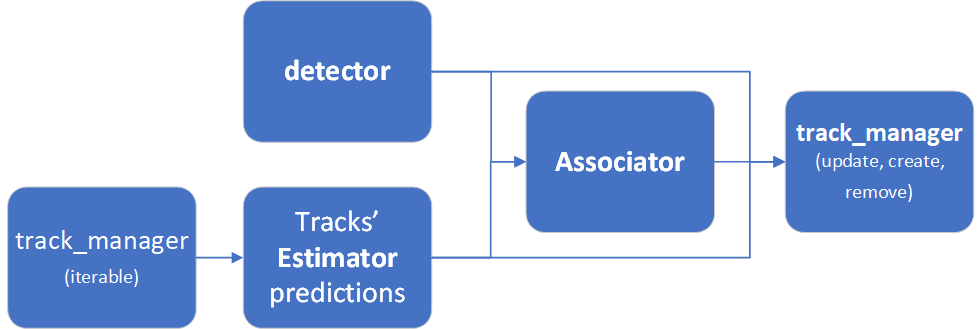
\includegraphics[width=0.9\linewidth]{figures/04_state_of_the_art/SORT.png}
    \caption[SORT algorithm]{\footnotesize{Block diagram of the SORT algorithm.}}
    \label{fig:sort}
    %\vspace{-1em}
\end{figure}

{
    \ac{SORT}\cite{Bewley2016_sort} is a model published in 2016, it reached competitive accuracies and speed simultaneously. 
    As it can be seen from the block diagram of the figure \ref{fig:sort}, the authors propose to use a system with the following four components:
}

\begin{enumerate}
    \item \textbf{Detector}: The detector solves the problem of finding an undefined number of regions that fit with a set of target objects within an image (frame). 
    The authors of \ac{SORT} use a \ac{CNN} based model that yields better detections than previous models, this reduce the estimations noise.
    \item \textbf{Estimator}: The estimator employs a Kalman filter, a recursive filter, to estimate the movement of each individual object based on noisy observations.
    \item \textbf{Associator}: The associator resolves the matching of the current frame detections with the active tracks estimations. The usage of a \ac{IoU} distance matrix and the Hungarian algorithm improved the speed with respect other systems.
    \item \textbf{Track manager}: The track manager creates and deletes the tracks given the other components results.
\end{enumerate}

%\needspace{0.1\textheight}

\paragraph{Detector}

{
    An operation that, given an input image, returns a set of output vectors containing the confidence, the object position, the object dimension and the class probability.
}

%\begin{equation}
%    \label{eqn:Detector definition}
%    Detector(I) = \{b_{0}, b_{1}, \hdots, b_{n}\} \; with \; b_{n} = \begin{bmatrix}
%        c \\
%        x \\
%        y \\
%        h \\
%        w \\
%        p_{c}
%      \end{bmatrix}
%\end{equation}
%
%\needspace{0.1\textheight}

\paragraph{Estimator}

{
    The \textbf{Kalman filter}\cite{kalman1960} operates in two main steps: prediction and updating.
    The prediction step estimates the \textbf{state mean} $x$ and covariance matrix $\mathbf{P}$ with the state transition matrix $\mathbf{F}$ and the process noise matrix $\mathbf{Q}$:
}
\begin{equation}
    \label{eqn:Kalman state mean estimation}
    \hat{x}_{k} = \mathbf{F} \cdot x_{k-1}
%    \hat{x}_{k} = \mathbf{F} \cdot x_{k-1} \; \; with \; x = \begin{bmatrix}
%        u \\
%        v \\
%        s \\
%        r \\
%        \dot u \\
%        \dot v \\
%        \dot s
%      \end{bmatrix}
\end{equation}

\begin{equation}
    \label{eqn:Kalman covariance matrix estimation}
    \hat{\mathbf{P}}_{k} = \mathbf{F} \cdot \mathbf{P}_{k-1} \cdot \mathbf{F}^{T} + \mathbf{Q}
\end{equation}

%{
%    Where $u \; and \; v$ is the object center, $s$ is the object scale, $r$ is the object aspect ratio and $\dot u, \dot v \; and \; \dot s$ are their velocities.
%}

{
    And, the updating step requires an observation $z$ (modified detection matched by the associator) 
    to correct the estimated state mean $x$ and covariance matrix $\mathbf{P}$ which improves the following iterations. 
    This is done with the Kalman gain $\mathbf{K}$, the measurements mask $\mathbf{H}$ and the measurements uncertainty matrix $\mathbf{R}$:
}

\begin{equation}
    \label{eqn:Kalman gain}
    \mathbf{K} = \hat{\mathbf{P}}_{k} \cdot \mathbf{H}^{T} \cdot (\mathbf{H} \cdot \mathbf{P}_{k} \cdot \mathbf{H}^{T} + \mathbf{R})^{-1}
\end{equation}

\begin{equation}
    \label{eqn:Kalman state mean correction}
    x_{k} = \hat{x}_{k} + \mathbf{K} \cdot (z - \mathbf{H} \cdot \hat{x}_{k})
%    x_{k} = \hat{x}_{k} + \mathbf{K} \cdot (z - \mathbf{H} \cdot \hat{x}_{k}) \; \; with \; z = \begin{bmatrix}
%        u\\ 
%        v\\ 
%        s\\ 
%        r
%        \end{bmatrix}
\end{equation}

\begin{equation}
    \label{eqn:Kalman covariance matrix correction}
    \mathbf{P}_{k} = (\mathbf{K} \cdot \mathbf{H})^{-1} \cdot \hat{\mathbf{P}}_{k} \cdot (\mathbf{K} \cdot \mathbf{H})^{-T} + \mathbf{K} \cdot \mathbf{R} \cdot \mathbf{K}^{T}
\end{equation}

\needspace{0.1\textheight}

\paragraph{Associator}

{
    The associator defines a \textbf{cost matrix} using negative \ac{IoU} between detections and estimations, with \ac{IoU} values below a certain threshold being rejected.
}

\begin{equation}
    \label{eqn:IoU}
    \begin{gathered}
        IoU(A, B) = \frac{|A \cap B|}{|A \cup B|} \\[0.25cm]
%        |A \cap B| = max(min_{x2}(A, B) - max_{x1}(A, B), 0) \cdot max(min_{y2}(A, B) - max_{y1}(A, B), 0) \\[0.25cm]
%        |A \cup B| = Area(A) + Area(B) - |A \cap B|
    \end{gathered}
\end{equation}

\needspace{0.1\textheight}

{
    The \textbf{Hungarian algorithm} associate the rows and columns assigning at most one row to each column and at most one column to each row with the minimum cost. 
    At the end, 3 sets are defined:
}

\begin{subequations}
    \begin{align}
        \mathit{A} = \{ (row, col) \mid (row, col) &\text{ is in the output of } Hungarian(-\mathbf{IoU}) \}
        \label{eqn:Assigned set} \\[0.5cm]
        \mathit{B} = \{ row &\mid \forall \: col \; \nexists \: (row, col) \in A \}
        \label{eqn:Unassigned detections set} \\[0.5cm]
        \mathit{C} = \{ col \mid& \; \forall \: row \; \nexists \: (row, col) \in A \}
        \label{eqn:Unassigned tracks set}
    \end{align}
\end{subequations}

\paragraph{Track manager}
{
    The Track Manager component uses the set of matched tracks and detections ($\mathit{A}$ in equation \ref{eqn:Assigned set}) 
    to update the Kalman filter for each assigned detection and track. 
    It also creates new potential tracks from unmatched detections ($\mathit{B}$ in equation \ref{eqn:Unassigned detections set}) 
    and potentially terminates tracks with missing associations ($\mathit{C}$ in equation \ref{eqn:Unassigned tracks set}).
}

{
    This model is the basis for subsequent tracking models discussed in this section.
}


\needspace{0.3\textheight}
\subsubsection{Deep SORT}


{
    Deep SORT\cite{Wojke2017simple} is a model published in 2017, it upgrades the SORT model with a new associator, containing appearance model.
}

\paragraph{Appearance model}

{
    The key innovation in Deep SORT is the introduction of an appearance model.
    The appearance model defines an operation that transforms the image crop with 
    the detected object in the image space into a new unitary norm feature space, 
    with the resulting feature vectors represented as $r_n$.
}

%\begin{equation}
%    \label{eqn:appearance model}
%    Appearance(crop(\mathbf{I}, b_{n})) = r_{n} \; \mid \; ||\:r_{n}\:|| = 1
%\end{equation}

\paragraph{Associator}

{
    The resulting feature space enables online identity definition using classical models such as \ac{KNN}, distance to the class mean or distance to the last instance.
    In the paper, the authors use the minimum cosine distance with the last 100 instances of each track as appearance distance, it is shown in the following equation \ref{eqn:cosine distance}.
}

\begin{equation}
    \label{eqn:cosine distance}
    d_{c}(i, j) = min\{1 - r_{j}^T \cdot r_{k}^{i} \;\mid\; r_{k}^{i} \in \text{"Last 100 appearances of identity i"} \}
\end{equation}

{
    The Deep SORT associator combines two distances: the location distance, represented by the Mahalanobis distance (equation \ref{eqn:Mahalanobis distance}), and the previous appearance distance. 
    The Mahalanobis distance considers the expected covariance between detections and track estimates. 
}

\begin{equation}
    \label{eqn:Mahalanobis distance}
    d_{m}(i, j) = (z_{j} - z_{i})^T \cdot P_{i}^{-1} \cdot (z_{j} - z_{i})
\end{equation}

{
    Here, $z_j$ is the $j$-th bounding box detection, and $z_i$ is the $i$-th track's bounding box estimation. 
    $P_i$ represents the covariance matrix estimation of the $i$-th track ($\hat{\mathbf{P}}_{k}$ in equation \ref{eqn:Kalman covariance matrix estimation}).
}

{
    The associator employs these distances to make inadmissible match discards. 
    The Mahalanobis distance can be thresholded using the inverse chi-squared ($\chi^2$) distribution, 
    while the appearance distance threshold can be data-driven.
}

{
    Subsequentially, both distances are combined using a weighted sum to make a cost matrix. 
    The authors argue in favor of using only the appearance distance. 
    This cost matrix is \textbf{split by track age} before applying linear assignments within a \textbf{matching cascade}, where recently tracked tracks are prioritized.
}

{
    Finally, a last assignment is done using a \ac{IoU} cost matrix computed from the unassigned detections and unassigned tracks of age 1 (recently tracked tracks and potential new tracks from the previous frame).
}



\needspace{0.18\textheight}
\subsubsection{ByteTrack}\label{sec:BYTE}


{
    \ac{BYTE}\cite{zhang2022bytetrack}, published in 2021, builds upon the SORT model with a two-staged associator and a deeper detector (YOLOX-X\cite{ge2021yolox}).
}

\paragraph{Associator}

{
    The two-staged associator divides \textbf{high confidence detections} from \textbf{low confidence detections}, 
    allowing for \textbf{different assignment criteria}.
    The authors propose either a combination of appearance for the high confidence and \ac{IoU} for the low confidence or \ac{IoU} for both stages.
}


\subsubsection{OC-SORT}


{
    \ac{OC-SORT}\cite{cao2023observation} is a 2021 model that builds upon the BYTE model. 
    It enhances the motion model, introduces an improved location score, and adds a third association stage, 
    excluding the appearance model for research purposes.
}

\paragraph{Motion model}

{
    In \ac{OC-SORT}, the Kalman filter is improved by freezing its state until a new observation is assigned. 
    The model updates each skipped frame using a linear model when new observations arrive (observation centric), 
    other models update their state with their own estimations (estimation centric). 
    \ac{SORT} is able to roughly follow a non-linear motion if the time between observations is short enough, 
    \ac{OC-SORT} reduce the estimation noise originated on missed frames.
} 

\paragraph{Location score}

{
    The location score from \ac{OC-SORT} is a global direction metric. 
    To compute this metric, \ac{OC-SORT} performs a search of the most relevant older observation:
    the oldest observation from the last $\Delta t=3$ frames, or the newest observation available.
    The relevant observation and the newest observation available are used to obtain the track global direction vector:
}

\begin{equation}
    \label{eqn:track direction}
    direction = \frac{(z_{new} - z_{old})}{||(z_{new} - z_{old})||}
\end{equation}

{
    A potential global direction is computed using the set of high score detections as potential new observations. 
    At the end, each track has its own global direction and the hypothetical global direction in the case of using a certain new detection.
}

%\begin{subequations}
%    \begin{align}
%        \mathbf{\Delta x_{tracks}} &= \begin{bmatrix}
%            direction_{1}[x] & direction_{1}[x] & \hdots & direction_{1}[x] \\
%            direction_{2}[x] & direction_{2}[x] & \hdots & direction_{2}[x] \\
%            \vdots & \vdots & \vdots & \vdots \\
%            direction_{M}[x] & direction_{M}[x] & \hdots & direction_{M}[x]
%            \end{bmatrix}
%        \label{eqn:dirction x tracks} \\[0.5cm]
%        \mathbf{\Delta y_{tracks}} &= \begin{bmatrix} \\
%            direction_{1}[y] & direction_{1}[y] & \hdots & direction_{1}[y] \\
%            direction_{2}[y] & direction_{2}[y] & \hdots & direction_{2}[y] \\
%            \vdots & \vdots & \vdots & \vdots \\
%            direction_{M}[y] & direction_{M}[y] & \hdots & direction_{M}[y]
%            \end{bmatrix}
%        \label{eqn:dirction y tracks} \\[0.5cm]
%        \mathbf{\Delta x_{detections}} &= \begin{bmatrix}
%            direction_{1,1}[x] & direction_{1,2}[x] & \hdots & direction_{1,N}[x] \\
%            direction_{2,1}[x] & direction_{2,2}[x] & \hdots & direction_{2,N}[x] \\
%            \vdots & \vdots & \vdots & \vdots \\
%            direction_{M,1}[x] & direction_{M,2}[x] & \hdots & direction_{M,N}[x]
%            \end{bmatrix}
%            \label{eqn:dirction x detections} \\[0.5cm]
%            \mathbf{\Delta y_{detections}} &= \begin{bmatrix}
%                direction_{1,1}[y] & direction_{1,2}[y] & \hdots & direction_{1,N}[y] \\
%                direction_{2,1}[y] & direction_{2,2}[y] & \hdots & direction_{2,N}[y] \\
%                \vdots & \vdots & \vdots & \vdots \\
%                direction_{M,1}[y] & direction_{M,2}[y] & \hdots & direction_{M,N}[y]
%            \end{bmatrix}
%            \label{eqn:dirction y detections}
%    \end{align}
%\end{subequations}

{
    These directions serve to obtain the angular distance $\mathbf{\Delta\phi}$ (from 0 to $\pi$) between the track and the detections trajectories, 
    later, it is transformed into a normalized angular score (from $-0.5$ to $0.5$) with the equation \ref{eqn:angular score}.
}


\begin{equation}
    \label{eqn:angular score}
%    \begin{split}
%        &\mathbf{\Delta\phi} = arccos(\Delta x_{tracks} \odot \Delta x_{detections} + \Delta y_{tracks} \odot \Delta y_{detections})\\
%        &\mathbf{\phi_{score}} = 0.5 - \left(\frac{|\mathbf{\Delta\phi}|}{\pi}\right)
%    \end{split}
    \mathbf{\phi_{score}} = 0.5 - \left(\frac{|\mathbf{\Delta\phi}|}{\pi}\right)
\end{equation}

\needspace{0.1\textheight}

\paragraph{Associator}

{
    During the association step, \ac{OC-SORT} categorizes the detections in three groups:
}

\begin{enumerate}
    \item Initially high score detections.
    \item Initially low score detections.
    \item High score associations that were not successfully associated
\end{enumerate}

{
    The first step performs a linear assignment with the Hungarian algorithm. 
    Using a weighted sum of the \ac{IoU} and the angular score from equation \ref{eqn:angular score} 
    pondered by the detections confidence ($c_{n}$) using the Hadamard product\footnote{The notation for element-wise product will be $\odot$ because $\oslash$ could be used for element-wise division.} as the cost:
}

\begin{equation}
    \label{eqn:detection confidence matrix}
    \mathbf{confidence_{detections}} = \begin{bmatrix}
        c_{1} & c_{2} & \hdots & c_{N} \\
        c_{1} & c_{2} & \hdots & c_{N} \\
        \vdots & \vdots & \vdots & \vdots \\ 
        c_{1} & c_{2} & \hdots & c_{N}
    \end{bmatrix}
\end{equation}

\begin{equation}
    \label{eqn:OC-SORT first association cost}
    cost_{1} = -\mathbf{IoU} - \lambda \cdot (\mathbf{\phi_{score}} \odot \mathbf{confidence_{detections}})
\end{equation}

{
    At the end of the first stage, a threshold on the \ac{IoU} is applied.
}

{
    The second association stage is the same as the \ac{BYTE} model (section \ref{sec:BYTE}): 
    the low confidence detections are assigned with a second location metric and threshold.
}
 
{
    The third stage of \ac{OC-SORT} is the same as the second stage; 
    however, it uses the last known observation of the remaining unmatched tracks and the remaining high confidence detections.
}

\subsubsection{Location metrics from OC-SORT}

{
    While not originally part of OC-SORT, the publicly available code from the OC-SORT authors includes a range of location metrics. 
    These metrics were initially developed for object detection but have found utility in object tracking scenarios, 
    particularly in improving the accuracy of associations compared to traditional \ac{IoU} by extending the overlapping ratio with a nearness ratio. 
    This section presents an exploration of three location metrics utilized in OC-SORT's codebase.
}

\paragraph{GIoU} 

{
    The \acl{GIoU}\cite{Rezatofighi_2018_CVPR} is a metric that extends the \ac{IoU} into the negatives and smoothen it by accounting for both positive and negative scenarios.
    However, it scores positively bigger boxes. 
    The upgrade consist in subtracting a term computed from the enclosure area and the complementary of the union with the enclosure area:
}


\begin{equation}
    \label{eqn:GIoU}
%    \begin{split}
%        GIoU(A, B) &= IoU(A, B) - \frac{|enclosure(A, B)| - |A \cup B|}{|enclosure(A, B)|} \\[0.25cm]
%        with \; |enclosure(A, B)| &= (max_{x2}(A, B) - min_{x1}(A, B)) \cdot (max_{y2}(A, B) - min_{y1}(A, B))
%    \end{split}
    GIoU(A, B) = IoU(A, B) - \frac{|enclosure(A, B)| - |A \cup B|}{|enclosure(A, B)|}
\end{equation}



\paragraph{DIoU} 

{
    The \acl{DIoU}\cite{Zheng_Wang_Liu_Li_Ye_Ren_2020} is a metric similar to the \ac{GIoU}, but with a different approach. 
    It replace the previous enclosure distance term with a the novel metric called \ac{IoO}. 
    \ac{IoO} is computed as the center distance normalized by the enclosure diagonal lenght:
}

\begin{equation}
    \label{eqn:DIoU}
    \begin{split}
        D&IoU(A, B) = IoU(A, B) - \frac{InnerDistance(A, B)}{OuterDistance(A, B)} \\[0.25cm]
        with& \; InnerDistance(A, B) = d(center(A), center(B)) \\[0.25cm]
        with& \; OuterDistance(A, B) = d(BottomRight(AB), UpperLeft(AB)) \\[0.25cm]
%        with& \; UpperLeft(AB) = [min_{x1}(A, B), min_{y1}(A, B)] \\[0.25cm]
%        with& \; BottomRight(AB) = [max_{x2}(A, B), max_{y2}(A, B)] \\[0.25cm]
%        with& \; d(P_{1}, P_{2}) = \sqrt{(P_{2_{x}} - P_{1_{x}})^{2} + (P_{2_{x}} - P_{1_{x}})^{2}}\\[0.25cm]
        &\text{using AB as a shortened notation for enclosure(A, B)}
    \end{split}
\end{equation}

\paragraph{CIoU}

{
    The \acl{CIoU}\cite{zheng2021ciou}, also from the same authors as \ac{DIoU}, further refines object association by accounting for variations in aspect ratios. 
    This new feature requires the computation of an aspect ratio distance, the authors uses a normalized quadratic angular distance, and an additional cost value based in the IoU. 
    The \ac{CIoU} score is defined as:
}

\begin{equation}
    \label{eqn:CIoU}
    \begin{split}
        C&IoU(A, B) = DIoU(A, B) - AspectRatioDistance(A, B) \cdot AspectRatioCost(A, B) \\[0.25cm]
        with& \; AspectRatioDistance(A, B) = \frac{4}{\pi^2} \cdot \left(arctan\left(\frac{B_{w}}{B_{h}}\right) - arctan\left(\frac{A_{w}}{A_{h}}\right)\right)^{2} \\[0.25cm]
        with& \; AspectRatioCost(A, B) = \frac{AspectRatioDistance(A, B)}{AspectRatioDistance(A, B) + 1 - IoU}
    \end{split}
\end{equation}


\subsubsection{Strong SORT}


{
    Strong SORT\cite{du2023strongsort} is a model published in 2022, 
    it upgrades the Deep SORT model, 
    introducing several notable features and improvements:
}

\begin{itemize}
    \item {
        \textbf{Advanced Modules}: 
        In contrast to Deep SORT, which employs a Faster R-CNN\cite{7485869, s23156887} for detection and a simple \ac{CNN} for appearance modeling, 
        Strong SORT employs more advanced models for both tasks. 
        Specifically, it utilizes YOLOX-X for detection and a \ac{BoT}\cite{Luo_2019_CVPR_Workshops} for appearance.
    }
    \item {
        \textbf{\ac{EMA}}: 
        Instead of maintaining a memory of the last 100 instances for the appearance model of each track, Strong SORT uses an exponential moving average.
    }
    \item {
        \textbf{\ac{ECC}}: 
        While Strong SORT includes a camera movement compensation model, 
        this feature is not relevant to the objectives of this project.
    }
    \item {
        \textbf{NSA Kalman}: 
        An improvement of the Kalman filter that estimates the measurements noise covariance using the detection confidence score.
    }
    \item {
        \textbf{Motion Cost}: 
        While Deep SORT assigns a weight of 1 on appearance and 0 on motion for track association, 
        Strong SORT suggests a weight of 0.98 on appearance and 0.02 on motion.
    }
    \item {
        \textbf{Vanilla Matching}: Strong SORT departs from the policy of prioritizing the recently tracked tracks during matching.
    }
    \item {
        \textbf{AFLink}: 
        An appearance-free deep learning model to postprocess results by joining tracklets\footnote{Tracklet (neologism): Continuous fragment of a track.}. 
        Note that it requires a substantial amount of training data.
    }
    \item {
        \textbf{\ac{GSI}}: 
        A space-temporal interpolator to fill the gaps caused by missing detections. 
        It employs a Gaussian process regression to model nonlinear motion.
    }
\end{itemize}

\paragraph{\acl{GSI}}

{
    The \ac{GSI} describes the i-th trajectory position $p_{t}$ at the time $t$ as a Gaussian process with kernel $k(x, x')$ and Gaussian noise $\varepsilon$:
}

\begin{equation}
    \label{eqn:gaussian trajectory}
    \begin{split}
        &p_{t} = f^{(i)}(t) + \varepsilon \\[0.25cm]
        with \;& f^{(i)} \in GP\left(0,\: k(\cdot,\cdot)\right) \\[0.25cm]
        with \;& \varepsilon \sim N\left(0,\: \sigma^{2}\right) \\[0.25cm]
        with \;& k(x, x') = e^{-\frac{||x - x'||^{2}}{2 \cdot \lambda{2}}}
    \end{split}
\end{equation}

\needspace{0.1\textheight}

{
    The predicted nonlinear positions $P^{*}$ (smoothed gap filled track) are obtained by fitting the linear predicted positions $P$ (gap filled track) into the previous Gaussian model trained per each track:
}


\begin{equation}
    \label{eqn:gaussian trajectory smoothing}
    \begin{split}
        &\mathbf{P^{*}} = \mathbf{K(F^{*}, F)} \cdot \left(\mathbf{K(F^{*}, F)} + \sigma^{2} \cdot \mathbf{I}\right)^{-1} \cdot \mathbf{P} \\[0.25cm]
        with \;& K(\cdot, \cdot) \text{ as the covariance function based on } k(\cdot, \cdot)
    \end{split}
\end{equation}


{
    Because this project only uses the \ac{GSI} from Strong SORT, the other features were briefly explained.
}



\subsubsection{Deep OC-SORT}


{
    Deep OC-SORT\cite{maggiolino2023deep} is a model published in 2023, 
    it builds upon the \ac{OC-SORT} model with the incorporation of an appearance model. 
    Although it also includes a feature for camera motion compensation (CMC), 
    this particular functionality is not within the scope of relevance for this project.
}

\paragraph{Appearance model}

{
    Similar to the Strong SORT model, Deep OC-SORT employs the \ac{BoT} model for extracting appearance embeddings ($e_{t}$) for each detection.
    However, Deep OC-SORT uses a new tracking by detection oriented moving average as a track representation; 
    it is a dynamic moving average influenced by the detection confidence ($s_{det}$), the detection acceptance threshold ($\sigma$), and a constant minimum weight of the previous memory ($\alpha_{f}$):
}

\begin{equation}
    \label{eqn:dynamic exponential moving average}
    \begin{split}
        &e_{t} = \alpha_{t} \cdot e_{t-1} + (1 - \alpha_{t}) \cdot e^{new} \\[0.25cm]
        with \;& \alpha_{t} = \alpha_{f} + (1 - \alpha_{f}) \cdot \left(1 - \frac{s_{det} - \sigma}{1 - \sigma}\right) \\[0.25cm]
        \text{when } s_{det} = \sigma : \;& \alpha_{t} = 1 \rightarrow e_{t} = e_{t-1} \\[0.25cm]
        \text{when } s_{det} = 1 : \;& \alpha_{t} = \alpha_{f} \rightarrow e_{t} = \alpha_{f} \cdot e_{t-1} + (1 - \alpha_{f}) \cdot e^{new}
    \end{split}
\end{equation}

{
    This dynamic appearance memory mitigates the impact from low quality frames (for example, a blurred object) and instances of occlusions during the tracked trajectory.
}

\paragraph{Associator}

{
    For the task of associating tracks with new detections, Deep OC-SORT employs a method involving cosine similarity. 
    This method results in the creation of an appearance matrix ($A_{c}$). 
}

{
    Like Deep SORT, this similarity is combined with the \ac{IoU} through a weighted sum to obtain the association cost matrix. 
    What distinguishes Deep OC-SORT is its introduction of an individual appearance weight for each pair of tracks and detections. 
    These weights are computed based on the discriminativeness\footnote{Discriminativeness: The authors of Deep OC-SORT use this word to refer to the quantification of discriminability.} of the appearance data.
}

{
    In the context of Deep OC-SORT, the authors define the discriminativeness 
    ($z_{diff}$) as the upper clipped difference of the highest and second highest score of each row or column (low scoring matches are irrelevant) of the appearance matrix ($A_{c}$).
    The mean of row discriminativeness and column discriminativeness plus a base weight ($a_{w}$) is their adaptive appearance weight:
}


\begin{equation}
    \label{eqn:adaptive appearance weight}
    \begin{split}
        &w(m, n) = a_{w} + \frac{z_{diff}^{track}(\mathbf{A_{c}}, m) + z_{diff}^{det}(\mathbf{A_{c}}, n)}{2} \\[0.25cm]
        with \;& z_{diff}^{track}(A_{c}, m) = \min\left( \max_{i} \left( \mathbf{A_{c}}[m, i] \right) - \max_{j \neq i} \left( \mathbf{A_{c}}[m, j] \right), \epsilon \right) \\[0.25cm]
        with \;& z_{diff}^{det}(A_{c}, n) = \min\left( \max_{i} \left( \mathbf{A_{c}}[i, n] \right)  - \max_{j \neq i} \left( \mathbf{A_{c}}[j, n] \right), \epsilon \right)
    \end{split}
\end{equation}


